\documentclass[11pt,a4paper]{article}

% --- Mathematics (must precede unicode-math) ---
\usepackage{amsmath}
\usepackage{mathtools}

% --- Fonts (lualatex) ---
\usepackage{fontspec}
\usepackage{unicode-math}
\setmathfont{KpMath-Regular.otf}
\setmathfont{KpMath-Bold.otf}[version=bold]

\usepackage{microtype}
\usepackage[dvipsnames]{xcolor}
\usepackage[margin=25mm, top=30mm, bottom=30mm]{geometry}

\usepackage{fancyhdr}
\pagestyle{fancy}
\fancyhf{}
\fancyhead[L]{\small\itshape Graded Voxels in Three Dimensions}
\fancyhead[R]{\small\itshape Nestor (2026)}
\fancyfoot[C]{\thepage}
\renewcommand{\headrulewidth}{0.4pt}
\renewcommand{\footrulewidth}{0pt}

\setcounter{secnumdepth}{3}
\usepackage{booktabs}
\usepackage{array}
\usepackage{graphicx}
\usepackage{placeins}
\usepackage[numbers,sort&compress]{natbib}
\usepackage[font=small, labelfont=bf, labelsep=period]{caption}
\usepackage{setspace}
\setstretch{1.15}
\setlength{\parskip}{0.4em}
\usepackage[colorlinks=true, linkcolor=blue!60!black,
            citecolor=blue!60!black, urlcolor=blue!60!black]{hyperref}

% --- Macros ---
\newcommand{\bI}{\mathbf{I}}
\newcommand{\bK}{\mathbf{K}}
\newcommand{\bM}{\mathbf{M}}
\newcommand{\bE}{\mathbf{E}}
\newcommand{\bP}{\mathbf{P}}
\newcommand{\bT}{\mathbf{T}}
\newcommand{\bW}{\mathbf{W}}
\newcommand{\bD}{\boldsymbol{\Delta}}
\newcommand{\sinc}{\operatorname{sinc}}
\newcommand{\nb}[1]{\texttt{#1}}
% the differential of every integral and derivative is upright: \dd z, \dd^2x, \frac{\dd}{\dd z};
% an italic d is the lattice pitch.
\newcommand{\dd}{\mathrm{d}}

\title{\bfseries Graded Voxels in Three Dimensions\\[4pt]
\large Galerkin Cubes with a Polynomial Field and Contrast:\\
the Source of their Error, its Cure, and Closed-Form Moment Integrals}
\author{T. M. Nestor\\[2pt]\small Independent researcher, Australia}
\date{1 October 2026}

\begin{document}
\maketitle

\begin{abstract}
\noindent
Voxel schemes represent a heterogeneous elastic medium as cells of constant properties, and in a smoothly
varying medium that representation caps them at second order in the cell size whatever the cell carries.
We build Galerkin cubes that carry polynomial moments of the nine-component state, displacement and an
independent strain, with a contrast that is itself a polynomial in the cell: first the cube with a
linear field and a linear contrast, then the one with both quadratic. On a sphere whose contrast falls
smoothly to zero at its surface, against its exact solution, the linear cube's discretisation converges at
fourth order (apparent orders $4.01$ and $4.13$) where uniform-field voxels converge at second, and at
full contrast its error is $42$ to $66$ times below the collocation voxel at the same cell size. Its
full-contrast order approaches four slowly, and we identify why. The error of the multiple-scattering term
is static, and it equals, to within $6\%$ on every grid, profile and shell width tried, the defect of the
$L^2$ projection of the contrast profile onto the cell's field functions: the once-scattered field has a
local part proportional to the contrast, and the cell can hold only its projection. Raising the degree of
the contrast alone gains $8\%$; raising the degree of the field as well removes the defect at that order.
The quadratic cube is more accurate than the linear one by factors of $4.1$, $6.0$, $10.0$, $15.6$ and
$20.8$ at $4$ to $12$ cells across, where the ratio of the two defects, computed from the profile alone,
is $4.4$, $6.2$, $9.8$, $15.6$ and $20.6$; it reaches with $408$ cells the accuracy the linear cube
reaches with $2{,}776$. The coupling blocks of the self cell and its neighbours are obtained in closed
form: a power series in the wavenumber whose coefficients are universal numbers, each a finite sum of
three elementary master integrals reduced from volume to faces to edges, derived here in full and checked
against the cube's Coulomb energy, the solid angle of the octant, an exact subdivision identity and
independent quadrature. The far-field extraction must treat the engineering shear stress of the source
consistently with the coupling kernel; a factor of two there is invisible at Born order along a cell axis.
\end{abstract}

\section{Introduction}\label{sec:intro}

A voxel scheme for elastic scattering replaces a heterogeneous body by cubic cells, each carrying a
single-site $T$-matrix and coupled through the background Green's tensor. In a layer of such cells the
scheme converges at second order when each cell carries a uniform internal field, and a cell that also
carries the first moment of its field converges at fourth order \citep{NestorContinuum2026}. That paper
also showed that where the medium varies within a cell, a contrast sampled as constant caps every
voxel at second order, and that the rule for a cell whose field has Legendre degree $p$ and whose
contrast has degree $r$ is $\min(2p+2,2r+2)$. All of that is one-dimensional, or three-dimensional only
for a laterally uniform layer, where the lateral moments are never excited.

This paper builds the three-dimensional graded cell and asks what it achieves on a body with genuine
three-dimensional structure: a sphere whose contrast falls smoothly to zero at its surface, which has an
exact solution and no staircase. It has three results. The cell with a linear field and a linear contrast
($p=r=1$) keeps the fourth order of its discretisation. Its error at full contrast is traced to a single
source, the defect of the projection of the contrast onto the cell's field functions, and that source is
removed by the cell with a quadratic field and contrast ($p=r=2$), so that far fewer cells give the same
accuracy. And the singular integrals on which both cells rest are obtained in closed form. The cell and
its single-site $T$-matrix are described in \S\ref{sec:voxel} and \S\ref{sec:site}, the coupling between
cells in \S\ref{sec:coupling}, the closed-form moments in \S\ref{sec:moments}, and the sphere in
\S\ref{sec:sphere}.

\section{The graded voxel}\label{sec:voxel}

A voxel is a cube $V=[-h,h]^3$ of half-width $h$ centred at $\mathbf{x}_c$, with local coordinates
$\boldsymbol{\xi}=(\mathbf{x}-\mathbf{x}_c)/h\in[-1,1]^3$ in the axis order $(z,x,y)$. The field in it is the
nine-component state $\psi=(\mathbf{u},\boldsymbol{\varepsilon})$: the displacement $\mathbf{u}$ and the
engineering strain $\boldsymbol{\varepsilon}$ in Voigt order $(zz,xx,yy,2xy,2zy,2zx)$. The strain is an
\emph{independent} unknown, not the gradient of $\mathbf{u}$. A basis whose strain is derived from its
displacement leaves a spurious source at every face between cells, because each cell's projected
displacement jumps across the face; in a layer that scheme converges at second or third order however
rich the basis \citep{NestorContinuum2026}. The quadratic 27-mode cube $T$-matrix is of that kind and is
not considered further.

The state is expanded in the Legendre polynomials of degree at most one,
\begin{equation}\label{eq:basis}
  \psi(\mathbf{x}) = \sum_{a=0}^{3}\psi_a\,L_a(\boldsymbol{\xi}),\qquad
  L_0=1,\quad L_i=\xi_{i-1}\ (i=1,2,3),
\end{equation}
36 weights per cell. The contrast operator
$\bD=\operatorname{diag}(\omega^2\Delta\rho\,\bI_3,\ \Delta\mathbf{C})$, with $\omega$ the angular
frequency, $\Delta\rho$ the density contrast and $\Delta\mathbf{C}$ the $6\times6$ Voigt stiffness
contrast, is linear in the cell,
\begin{equation}\label{eq:contrast}
  \bD(\boldsymbol{\xi}) = \bD_0+\sum_{i=1}^{3}\bD_i\,\xi_{i-1},
\end{equation}
its coefficients the $L^2$ projection of the medium onto $\{1,\xi_i\}$. The source density
$\bD\psi$ is then a polynomial of degree at most two. Writing $m_c$ ($c=0,\dots,9$) for the ten monomials
of degree at most two,
\begin{equation}\label{eq:linearisation}
  \bD(\boldsymbol{\xi})\,L_b(\boldsymbol{\xi})=\sum_{c=0}^{9}\bE_{cb}\,m_c(\boldsymbol{\xi}),
\end{equation}
where $\bE_{cb}$ collects the $9\times9$ coefficients: the Legendre linearisation of the one-dimensional
construction \citep{NestorContinuum2026}, with no new kernel object. The Lippmann--Schwinger equation
$\psi=\psi^0+\int\bP(\mathbf{x}-\mathbf{x}')\,\bD\psi\,\dd^3x'$, with $\psi^0$ the incident state and
$\bP$ the $9\times9$ point propagator $[[\mathbf{G},\mathbf{C}],[\mathbf{H},\mathbf{S}]]$ built from the
elastodynamic Green's tensor and its derivatives, is tested with each $L_a$ over each cell (Galerkin).
Cells $m$ and $n$ couple through the blocks
\begin{equation}\label{eq:block}
  \bK_{ac}(\mathbf{R}) = \int_{V_m}\!\int_{V_n} L_a(\boldsymbol{\xi})\,
  \bP(\mathbf{x}-\mathbf{x}')\,m_c(\boldsymbol{\xi}')\,\dd^3x\,\dd^3x',\qquad \mathbf{R}=\mathbf{x}_m-\mathbf{x}_n,
\end{equation}
and the discrete system is
\begin{equation}\label{eq:system}
  \sum_b\bM_{ab}\psi_{m,b}-\sum_n\sum_{b,c}\bK_{ac}(\mathbf{R}_{mn})\,\bE^{(n)}_{cb}\,\psi_{n,b}
  =\langle L_a,\psi^0\rangle_m ,
\end{equation}
with $\bM_{ab}=\langle L_a,L_b\rangle\,\bI_9$ the Gram matrix,
$\operatorname{diag}(8h^3,\,8h^3/3,\,8h^3/3,\,8h^3/3)$.

\paragraph{Higher degree.} Nothing in the construction is particular to degree one. The ten polynomials
\begin{equation}\label{eq:qbasis}
  Q_a\in\bigl\{1,\ \xi_i,\ \tfrac12(3\xi_i^2-1),\ \xi_i\xi_j\ (i<j)\bigr\}
\end{equation}
are orthogonal on the cell, with $\langle Q_a,Q_a\rangle=h^3\,(8,\tfrac83,\tfrac85,\tfrac89)$ by kind, and
their first four are the $L_a$. A contrast quadratic in the cell is the $L^2$ projection of the medium
onto all ten ($r=2$); a field quadratic in the cell is expanded in all ten ($p=2$), $90$ weights per cell.
The products $Q_aQ_b$ are expanded in monomials as in Eq.~\eqref{eq:linearisation}: $10$, $20$ or $35$
of them for a source of degree two, three or four. The blocks \eqref{eq:block} are computed with test
monomials and recombined into the $Q_a$, the first four rows and the first ten columns being those of the
linear cell. The incident moments are $\langle Q_a,\mathrm{e}^{\mathrm{i}\mathbf{k}\cdot\mathbf{x}}\rangle
=h^3\mathrm{e}^{\mathrm{i}\mathbf{k}\cdot\mathbf{x}_c}\prod_i2\,\mathrm{i}^{n_i}j_{n_i}(k_ih)$, with $n_i$
the Legendre degree of $Q_a$ on axis $i$ and $j_n$ the spherical Bessel function.

\section{The single site}\label{sec:site}

For one isolated cell the system closes on the self block $\bK(0)$. With the source moments
$\sigma_a=\langle L_a,\bD\psi\rangle=\sum_b\mathbf{F}_{ab}\psi_b$,
$\mathbf{F}_{ab}=\sum_c\langle L_a,m_c\rangle\bE_{cb}$, the graded single site is
\begin{equation}\label{eq:t36}
  \bT_{36}=\mathbf{F}\,\bigl(\bM-\bK(0)\,\bE\bigr)^{-1}\bM ,
\end{equation}
which maps the incident field's Legendre coefficients to the source moments: force and stress means and
their first moments. The first moment of the force, which a nine-component composite cannot hold, is part
of the object.

\paragraph{Parity.} Under inversion $\mathbf{x}\to-\mathbf{x}$ the displacement is odd, the strain even
and $\xi_i$ odd. With $g=0$ (no gradient) $\bT_{36}$ therefore splits exactly into a 15-dimensional set
(strain$\times1$, displacement$\times\xi$) and a 21-dimensional set (displacement$\times1$,
strain$\times\xi$); the coupling between them is $5\times10^{-18}$ of the largest entry. A gradient is odd
about the centre and couples the two sets linearly: $0.325\,gh$ of the largest entry, for a gradient $g$
along one axis, at $gh=0.05$, $0.1$ and $0.2$. An axis-aligned gradient leaves the symmetry of rotations by
a quarter turn about its axis, which $\bT_{36}$ satisfies to $10^{-11}$.

\paragraph{The inverse by symmetry.} The 36 unknowns carry the representation
$\mathbf{D}(\mathbf{Q})=\mathbf{T}(\mathbf{Q})\otimes\mathbf{S}(\mathbf{Q})$ of the 48 symmetries
$\mathbf{Q}$ of the cube, $\mathbf{T}$ acting on the functions $\{1,\xi_i\}$ and $\mathbf{S}$ on the nine
components (\S\ref{sec:sphere}). The self block has the full symmetry of the cube, and with a contrast
uniform in the cell so does $\mathbf{A}=\bM-\bK(0)\bE$: it commutes with every $\mathbf{D}(\mathbf{Q})$.
By Schur's lemma $\mathbf{A}$ is then an $n\times n$ block, repeated $d$ times, on each irreducible
representation of $O_h$ of dimension $d$ that occurs $n$ times, and the inverse in Eq.~\eqref{eq:t36} is
the inverse of those blocks (Table~\ref{tab:irreps}). The uniform strain ($1\times\boldsymbol\varepsilon$)
is $A_{1g}+E_g+T_{2g}$: dilatation, the two diagonal deviators and the three shears. The linear
displacement ($\xi\times\mathbf{u}$) is $A_{1g}+E_g+T_{1g}+T_{2g}$: the same three, which are the strain
of a linear displacement, and the rigid rotation $T_{1g}$. Each strain therefore pairs with its own
linear displacement in a $2\times2$ block, and the rotation stands alone. The odd set is the mean
displacement, $T_{1u}$, and the eighteen linear strains, $3T_{1u}+2T_{2u}+A_{2u}+E_u$. No block is larger
than $4\times4$, so $\bT_{36}$ of a uniform cell is available in closed form. Numerically
(\path{scripts/check_graded_voxel_site_symmetry.py}), $\mathbf{A}$ commutes with all 48 operations to
$10^{-16}$ of its largest entry; the multiplicities follow from the characters; on each representation
$\mathbf{A}$ has $n$ distinct eigenvalues, each $d$-fold; and the inverse assembled from the blocks equals
the $36\times36$ inverse to $10^{-15}$.

\begin{table}[ht]
\centering\small
\setlength{\tabcolsep}{7pt}
\begin{tabular}{@{}lcccccccc@{}}
\toprule
 & \multicolumn{4}{c}{even (15)} & \multicolumn{4}{c}{odd (21)} \\
\cmidrule(lr){2-5}\cmidrule(lr){6-9}
representation & $A_{1g}$ & $E_g$ & $T_{1g}$ & $T_{2g}$ & $A_{2u}$ & $E_u$ & $T_{1u}$ & $T_{2u}$ \\
\midrule
dimension $d$ & 1 & 2 & 3 & 3 & 1 & 2 & 3 & 3 \\
multiplicity $n$ (block $n\times n$) & 2 & 2 & 1 & 2 & 1 & 1 & 4 & 2 \\
\bottomrule
\end{tabular}
\caption{The single-site matrix of a cell with uniform contrast, reduced on the irreducible
representations of the cube group: $\sum nd=36$.}\label{tab:irreps}
\end{table}

\paragraph{The blocks, entry by entry.} In the static limit the contrast acts on the strain alone, so the
displacement-type functions drop out of $\mathbf{A}^{-1}$ wherever it meets $\bD$, and $\bT_{36}$ is carried
by the strain-type functions: the uniform strain ($A_{1g}+E_g+T_{2g}$) and the linear strain
($3T_{1u}+2T_{2u}+A_{2u}+E_u$). On each representation $\Gamma$,
\begin{equation}\label{eq:tblock}
  \bT_\Gamma=M_\Gamma\,\boldsymbol\Delta_\Gamma\bigl(\bI-\mathbf{N}_\Gamma\boldsymbol\Delta_\Gamma\bigr)^{-1},
  \qquad \mathbf{N}_\Gamma=M_\Gamma^{-1}\bK_\Gamma=\frac{1}{\mu}\bigl(\mathbf{p}_\Gamma+b_2\,\mathbf{q}_\Gamma\bigr),
\end{equation}
with $M_\Gamma=8h^3$ for the uniform strain and $8h^3/3$ for the linear, $b_2=-\tfrac12(1-\beta^2/\alpha^2)$,
and $\boldsymbol\Delta_\Gamma$ the contrast on the representation. The numbers $\mathbf{p}_\Gamma$ and
$\mathbf{q}_\Gamma$ are the two families of Eq.~\eqref{eq:series} (the $\delta_{ij}/r$ and the
$\partial_i\partial_jr$ parts of the Kelvin tensor). They do not depend on $h$, and they are rational
combinations of five constants,
\begin{equation}\label{eq:fiveconstants}
  1,\qquad \frac1\pi,\qquad \frac{\sqrt2}{\pi},\qquad \frac{\sqrt3}{\pi},\qquad
  \Lambda=\frac{1}{\pi}\Bigl[\ln\bigl(1+\sqrt2\bigr)-\operatorname{arsinh}\frac{1}{\sqrt2}\Bigr],
\end{equation}
obtained by carrying the reductions of \S\ref{sec:moments} in exact arithmetic. With $\gamma_{ij}$ the
engineering shear on axes $i,j$, the representations are spanned, for the partner along axis $0$, by
\begin{equation*}
\begin{array}{@{}ll@{\qquad}ll@{}}
  A_{1g}: & \varepsilon_{00}+\varepsilon_{11}+\varepsilon_{22}, & E_g: & 2\varepsilon_{00}-\varepsilon_{11}-\varepsilon_{22},\\[2pt]
  T_{2g}: & \gamma_{12}, & A_{2u}: & \xi_0\gamma_{12}+\xi_1\gamma_{02}+\xi_2\gamma_{01},\\[2pt]
  T_{1u}: & \multicolumn{3}{@{}l@{}}{v_1=\xi_0\varepsilon_{00},\quad v_2=\xi_0(\varepsilon_{11}+\varepsilon_{22}),\quad
            v_3=\xi_1\gamma_{01}+\xi_2\gamma_{02},}\\[2pt]
  T_{2u}: & \multicolumn{3}{@{}l@{}}{w_1=\xi_0(\varepsilon_{11}-\varepsilon_{22}),\quad w_2=\xi_1\gamma_{01}-\xi_2\gamma_{02},}\\[2pt]
  E_u: & \xi_1\gamma_{02}-\xi_2\gamma_{01}, & &
\end{array}
\end{equation*}
and the blocks are the matrices of the operators in these vectors (they are not normalised, so the blocks
are not symmetric). The contrast is $\boldsymbol\Delta=3\Delta\lambda+2\Delta\mu$ on $A_{1g}$, $2\Delta\mu$
on every other one-dimensional block and on $T_{2u}$, and on $T_{1u}$
\begin{equation}
  \boldsymbol\Delta_{T_{1u}}=\begin{pmatrix}\Delta\lambda+2\Delta\mu&2\Delta\lambda&0\\
  \Delta\lambda&2\Delta\lambda+2\Delta\mu&0\\0&0&2\Delta\mu\end{pmatrix}.
\end{equation}
For the uniform strain,
\begin{equation}\label{eq:uniformblocks}
  N_{A_{1g}}=-\frac{1+2b_2}{3\mu}=-\frac{1}{3(\lambda+2\mu)},\qquad
  N_{E_g}=-\frac{1}{3\mu}+\frac{b_2}{\mu}\Bigl(3c_1-\frac23\Bigr),\qquad
  N_{T_{2g}}=-\frac{1}{3\mu}-\frac{2b_2c_1}{\mu},
\end{equation}
with $c_1=(1-2\sqrt2+\sqrt3)/\pi+2\Lambda=0.111222$. The dilatation is that of any shape. The two shear
entries satisfy $2q_{E_g}+3q_{T_{2g}}=-\tfrac43$, the sphere's value $-\tfrac{4}{15}$ on each of the five
deviators: the cube splits them $3{:}2$ about the sphere. For the linear strain the first family is one
more constant,
\begin{equation}
  c_0=\frac{2-3\sqrt2+\sqrt3}{5\pi}+\Lambda=0.038444,
\end{equation}
and Table~\ref{tab:blocks} lists every entry. Assembled with Eq.~\eqref{eq:tblock}, these blocks reproduce
the strain rows of the $36\times36$ single site as $\omega\to0$ to $5\times10^{-16}$, and the exact
moments agree with the 40-digit ones of \S\ref{sec:moments} to $10^{-14}$
(\path{scripts/derive_graded_voxel_site_blocks.py}). At finite frequency the displacement-type functions
enter at order $(k_Sh)^2$ through the terms $m\ge0$ of Eq.~\eqref{eq:series}, built from the same moments;
those entries are not tabulated here.

\begin{table}[ht]
\centering\small
\setlength{\tabcolsep}{5pt}
\begin{tabular}{@{}llcrrrrr@{}}
\toprule
 & & & \multicolumn{5}{c}{$q$: coefficient of} \\
\cmidrule(lr){4-8}
block & entry & $p$ & $1$ & $1/\pi$ & $\sqrt2/\pi$ & $\sqrt3/\pi$ & $\Lambda$ \\
\midrule
$T_{1u}$ & $(1,1)$ & $-\tfrac13-8c_0$ & $-\tfrac23$ & $-\tfrac{14}{5}$ & $\tfrac{36}{5}$ & $-\tfrac{22}{5}$ & $-4$ \\
 & $(1,2)$ & $0$ & $0$ & $-\tfrac{18}{5}$ & $\tfrac{12}{5}$ & $\tfrac65$ & $-12$ \\
 & $(1,3)$ & $-\tfrac16+2c_0$ & $-\tfrac23$ & $\tfrac{22}{5}$ & $-\tfrac{48}{5}$ & $\tfrac{26}{5}$ & $8$ \\
 & $(2,1)$ & $0$ & $0$ & $-\tfrac95$ & $\tfrac65$ & $\tfrac35$ & $-6$ \\
 & $(2,2)$ & $-\tfrac13+4c_0$ & $-\tfrac23$ & $5$ & $-6$ & $1$ & $14$ \\
 & $(2,3)$ & $-\tfrac1{12}+c_0$ & $0$ & $-\tfrac35$ & $\tfrac{12}{5}$ & $-\tfrac95$ & $0$ \\
 & $(3,1)$ & $-\tfrac16+2c_0$ & $-\tfrac23$ & $\tfrac{22}{5}$ & $-\tfrac{48}{5}$ & $\tfrac{26}{5}$ & $8$ \\
 & $(3,2)$ & $-\tfrac16+2c_0$ & $0$ & $-\tfrac65$ & $\tfrac{24}{5}$ & $-\tfrac{18}{5}$ & $0$ \\
 & $(3,3)$ & $-\tfrac5{12}-c_0$ & $\tfrac23$ & $-\tfrac{46}{5}$ & $\tfrac{84}{5}$ & $-\tfrac{38}{5}$ & $-20$ \\
\midrule
$T_{2u}$ & $(1,1)$ & $-\tfrac13+4c_0$ & $-\tfrac23$ & $\tfrac{233}{15}$ & $-\tfrac{422}{15}$ & $\tfrac{63}{5}$ & $18$ \\
 & $(1,2)$ & $-\tfrac1{12}+c_0$ & $-\tfrac23$ & $5$ & $-12$ & $7$ & $8$ \\
 & $(2,1)$ & $-\tfrac16+2c_0$ & $-\tfrac43$ & $10$ & $-24$ & $14$ & $16$ \\
 & $(2,2)$ & $-\tfrac14-3c_0$ & $-\tfrac23$ & $2$ & $-12$ & $10$ & $-4$ \\
\midrule
$A_{2u}$ & & $-\tfrac12+6c_0$ & $\tfrac43$ & $-\tfrac{326}{15}$ & $\tfrac{764}{15}$ & $-\tfrac{146}{5}$ & $-20$ \\
$E_u$ & & $-\tfrac14+3c_0$ & $-\tfrac23$ & $-\tfrac{74}{15}$ & $\tfrac{116}{15}$ & $-\tfrac{14}{5}$ & $4$ \\
\bottomrule
\end{tabular}
\caption{The static blocks of the linear strain in closed form: $\mathbf{N}_\Gamma=(\mathbf{p}+b_2\mathbf{q})/\mu$,
with $q$ given by its rational coefficients on the constants of Eq.~\eqref{eq:fiveconstants}. Rows and
columns of $T_{1u}$ are $(v_1,v_2,v_3)$, of $T_{2u}$ $(w_1,w_2)$.}\label{tab:blocks}
\end{table}

A gradient lowers the symmetry. With a gradient along a cell axis, exactly the eight operations that fix
the axis still commute with $\mathbf{A}$, and the reduction is on the representations of that smaller
group. In a general direction nothing is left but covariance: $\mathbf{D}(\mathbf{Q})$ carries the
single site of a cell to that of the cell with the rotated gradient, so cells whose gradients are related
by a symmetry of the cube share one inverse.

\paragraph{Reciprocity.} The propagator satisfies $\bW\bP(\mathbf{r})$ symmetric at every
$\mathbf{r}$, with $\bW=\operatorname{diag}(\bI_6,\tfrac12\bI_3)$, and
$\bP(-\mathbf{r})=\boldsymbol{\Pi}\bP(\mathbf{r})\boldsymbol{\Pi}$ with
$\boldsymbol{\Pi}=\operatorname{diag}(-\bI_3,\bI_6)$. Every block between test functions is therefore
$\bW$-symmetric, $(\bW\bK_{ab})^{\mathsf T}=\bW\bK_{ab}$, and the self block obeys
$\bK_{ba}(0)=\boldsymbol{\Pi}\bK_{ab}(0)\boldsymbol{\Pi}$ (exchange the two points of the cell). Both hold
to $10^{-11}$.

\paragraph{The Born limit.} Without a gradient $\bT_{36}$ is exact at first order in the contrast for any
incident field: the source moments are $\bD_0\langle L_a,\psi^0\rangle$. With a gradient the first-order
source $\langle L_a,(\mathbf{g}\cdot\boldsymbol{\xi})\psi^0\rangle$ needs the incident field's
\emph{quadratic} moments, which the degree-one input drops. The error is $O(\Delta\,gh\,(kh)^2)$, with $k$
the incident wavenumber: measured slopes $2.0001$ and $2.0004$ for $kh=0.025\to0.05\to0.1$, where it
reaches $8.9\times10^{-5}$ at $gh=0.2$ (these and the parity numbers: \path{scripts/measure_graded_voxel_site.py}).
It is the single site's view of the rule
$\min(2p+2,2r+2)$ for a field of degree $p$ and a contrast of degree $r$ \citep{NestorContinuum2026}.

\paragraph{An isolated cube has an error floor that refinement in $k$ does not remove.} In the static
limit a cube of contrast $\Delta\mathbf{C}$ under a uniform remote strain has the internal strain
$\boldsymbol{\varepsilon}(\mathbf{x})=\boldsymbol{\varepsilon}^0+\int_V\partial\partial\mathbf{G}(\mathbf{x}-\mathbf{x}')\,
\Delta\mathbf{C}\,\boldsymbol{\varepsilon}(\mathbf{x}')\,\dd^3x'$. The self-interaction
$\mathbf{S}(\mathbf{x})=\int_V\partial\partial\mathbf{G}(\mathbf{x}-\mathbf{x}')\,\dd^3x'$ is constant
inside an ellipsoid and only there \citep{Eshelby1957}; in a cube it concentrates towards the edges and
corners. A closure that keeps averages is exact through second order in the contrast, since the
second-order source needs only $\int_V\mathbf{S}$, and first errs at third order, by
$\Delta\mathbf{C}^3\,V\operatorname{Var}(\mathbf{S})$; a collocation closure, which uses
$\mathbf{S}(0)$, errs already at second order. Neither error depends on $k$. It is not what a tiled medium
sees: between identical cells the faces are not physical, the exact field is smooth there, and the
concentration does not arise. The order of convergence is a property of the tiled medium, the closure
error a property of the isolated cell; this paper measures the former
(\S\ref{sec:sphere}).

\section{The coupling between cells}\label{sec:coupling}

\paragraph{The point propagator.} $\bP$ is built from
$\mathbf{G}_{ij}=\frac{1}{4\pi\mu}\bigl[\delta_{ij}g_S(r)+k_S^{-2}\partial_i\partial_j(g_S-g_P)(r)\bigr]$,
$g_k=\mathrm{e}^{\mathrm{i}kr}/r$, with $\mu$ the background shear modulus and $k_P$, $k_S$ the P and S
wavenumbers. Every derivative of a radial function $f$ is a combination of
$F_q=(r^{-1}\dd/\dd r)^q f$. Near the origin the closed form cancels catastrophically (the
$k_S^{-2}$ difference), so for $k_Sr\le\tfrac12$ the $F_q$ are summed term by term from the power series
of $g_k$. This kernel equals the package's closed form to $10^{-11}$ where both are accurate, and its
static part is the Kelvin tensor to $10^{-13}$. Its static (Kelvin) part is the $t=0$ term of the
$\delta_{ij}$ series and the $t=2$ term of the derivative series, $\frac{1}{4\pi\mu}[\delta_{ij}r^{-1}
+b_2\partial_i\partial_jr]$ with $b_2=-\tfrac12(1-\beta^2/\alpha^2)$; the dynamic remainder is at most
$1/r$.

\paragraph{The $s$-form.} With $\mathbf{x}=\mathbf{x}_m+\mathbf{u}$ and $\mathbf{x}'=\mathbf{x}_n+\mathbf{u}'$
the kernel sees $\mathbf{R}+\mathbf{s}$, $\mathbf{s}=\mathbf{u}-\mathbf{u}'\in[-2h,2h]^3$, and
Eq.~\eqref{eq:block} becomes
\begin{equation}\label{eq:sform}
  \bK_{ac}(\mathbf{R})=\int W_{ac}(\mathbf{s})\,\bP(\mathbf{R}+\mathbf{s})\,\dd^3s,\qquad
  W_{ac}(\mathbf{s})=\prod_{i}w_{e_{a,i}e_{c,i}}(s_i),
\end{equation}
with the one-dimensional cross-correlation
$w_{\alpha\beta}(s)=h\int v^\alpha(v-s/h)^\beta\,\dd v$ over
$v\in[\max(-1,s/h-1),\min(1,s/h+1)]$: continuous, a polynomial on $[-2h,0]$ and on $[0,2h]$, zero at
$\pm2h$, with kinks at $0$ and $\pm2h$. For cells that do not touch the kernel is smooth on each of the
eight pieces and a three-dimensional Gauss rule suffices ($8n^3$ kernel evaluations against $n^6$ for the
double integral). It agrees with six-dimensional Gauss quadrature of Eq.~\eqref{eq:block} to $10^{-9}$ one
cell beyond contact.

\paragraph{The self cell and its 26 neighbours.} The static part is a sum of terms
$\partial^{\boldsymbol{\iota}}r^m$ ($m=-1$ with $|\boldsymbol{\iota}|\le2$, $m=1$ with
$|\boldsymbol{\iota}|\le4$), distributions at the origin. Moving
$k=\max(0,|\boldsymbol{\iota}|-(m+1))\le2$ derivatives onto $W$ leaves a kernel at most $1/r$:
$\int W\,\partial^{\boldsymbol{\iota}}f=(-1)^k\int(\partial^{\text{moved}}W)\,\partial^{\text{rest}}f$.
Two derivatives on one axis turn the kinks of $w$ into plane deltas $J_b\,\delta(s-bh)$,
$b\in\{-2,0,2\}$, $J_b$ the jump of $w'$ at $b$. Every piece is then a box or a rectangle whose corners
lie on the breakpoints, so the singular point $\mathbf{s}=-\mathbf{R}$ is either a vertex, integrated
with Duffy's pyramids, or at distance $2h$ or more. The Eshelby delta is not added by hand; it is carried by
the plane deltas. The construction reproduces the Eshelby sum rule
$\sum_p\int\!\!\int_{V\times V}\partial_p\partial_p r^{-1}=-4\pi V$ and the cube's Coulomb self-energy
\begin{equation}\label{eq:coulomb}
  \int\!\!\int_{V\times V}\frac{\dd^3x\,\dd^3x'}{|\mathbf{x}-\mathbf{x}'|}
  =2\Bigl[\tfrac15\bigl(1+\sqrt2-2\sqrt3\bigr)-\tfrac{\pi}{3}+\ln\bigl((1+\sqrt2)(2+\sqrt3)\bigr)\Bigr](2h)^5
\end{equation}
to $10^{-11}$, converges in the Gauss order to $10^{-11}$, and satisfies the reciprocity and exchange laws
of \S\ref{sec:site}. The biharmonic rule $\sum_{p,q}\partial_p\partial_p\partial_q\partial_q r=-8\pi\delta$
holds to the same accuracy, which checks the delta carried by the $r$ terms. And every block equals the
sum of the $64$ blocks between the two cells' half-size sub-cells, with the polynomials re-expressed on the
sub-cells, to $2\times10^{-15}$ for all $(a,c)$ at the self cell, its touching neighbours and beyond
(\path{scripts/check_graded_voxel_subdivision.py}).

The pieces are integrated here by quadrature; \S\ref{sec:moments} evaluates the same pieces in closed form.

\paragraph{An independent construction.} Integration by parts can move the derivatives onto the cells'
polynomials instead of onto $W$: one derivative onto each cell, each move either differentiating the
polynomial or producing a face term, which leaves $1/r$ kernels over cell$\times$cell, face$\times$cell
and face$\times$face, all absolutely convergent. Built in Mathematica on its own (\path{GradedVoxel_WeakKernel.wl}),
this reproduces the sum rule and the Coulomb energy, and, as the source cell shrinks to a point, the
distributional single average of the moment engine \citep{NestorContinuum2026}; all to $10^{-14}$ or
better.

\section{The moment integrals in closed form}\label{sec:moments}

The blocks of the self cell and of its 26 neighbours need no quadrature. They are a power series in the
wavenumber whose coefficients are pure numbers, each a finite sum of elementary master integrals. This
section derives them from the definition \eqref{eq:block}; nothing is taken from elsewhere.

\paragraph{The series in the wavenumber.} With $g_k=\mathrm{e}^{\mathrm{i}kr}/r=\sum_{t\ge0}(\mathrm{i}k)^t
r^{t-1}/t!$, the Green's tensor is a sum over powers $r^m$, $m=t-1\ge-1$, of two families,
\begin{equation}\label{eq:series}
  \mathbf{G}_{ij}=\frac{1}{4\pi\mu}\sum_{m\ge-1}\Bigl[c_1(m)\,\delta_{ij}\,r^m+c_2(m)\,\partial_i\partial_j r^m\Bigr],
  \qquad
  c_1=\frac{(\mathrm{i}k_S)^{m+1}}{(m+1)!},\quad
  c_2=\frac{\mathrm{i}^{m+1}\bigl(k_S^{m+1}-k_P^{m+1}\bigr)}{k_S^2\,(m+1)!}.
\end{equation}
The static (Kelvin) tensor is $c_1$ at $m=-1$ and $c_2$ at $m=1$, where $c_2=b_2$. The propagator $\bP$
adds up to two derivatives to $\mathbf{G}$, so every entry of every block is a sum of the scalar moments
\begin{equation}\label{eq:umoment}
  \int_{V_m}\!\int_{V_n}L_a\,\partial^{\boldsymbol\iota}r^m\,m_c\,\dd^3x\,\dd^3x'
  =h^{\,6+m-|\boldsymbol\iota|}\;U_{ac}(m,\boldsymbol\iota;\mathbf{o}),
  \qquad |\boldsymbol\iota|\le4,
\end{equation}
with $\mathbf{o}=\mathbf{R}/2h$ the integer offset between the cells. The $U$ are numbers: they depend on
neither the cell size, the frequency nor the medium. The medium enters a block only through $c_1$, $c_2$ and
two fixed tables of $9\times9$ integer matrices, one for each family, that say which entry of $\bP$ takes
which derivative $\partial^{\boldsymbol\iota}$. The series is that of the exponential and converges for
every $k$; for touching cells its term $t$ is bounded by $(4\sqrt3\,k_Sh)^t/t!$.

\paragraph{Even and odd powers.} For even $m$, $r^m$ is a polynomial and \eqref{eq:umoment} is an integral
of polynomials over the pieces of $W$, exact by a Gauss rule of sufficient order. For odd $m$ the kernel is
singular at $\mathbf{x}=\mathbf{x}'$, and for $m=\pm1$ with enough derivatives it is a distribution. Of the
derivatives in $\boldsymbol\iota$,
\begin{equation}\label{eq:moves}
  k=\max\Bigl(0,\;|\boldsymbol\iota|-\min\bigl(m+1,\tfrac{m+3}{2}\bigr)\Bigr)\le2
\end{equation}
are moved onto $W$ as in \S\ref{sec:coupling}. What remains, $\partial^{\text{rest}}r^m$, is then at most
$1/r$ singular, and it is a sum of monomials times odd powers of the distance no lower than $r^{-3}$, by
\begin{equation}\label{eq:monomials}
  \partial_i\bigl(t^{\boldsymbol\alpha}\,|t|^{n}\bigr)
  =\alpha_i\,t^{\boldsymbol\alpha-\mathbf{e}_i}\,|t|^{n}+n\,t^{\boldsymbol\alpha+\mathbf{e}_i}\,|t|^{n-2}:
\end{equation}
$1/r$ for $m=-1$, and $\delta_{ij}/r-t_it_j/r^3$ for $m=1$.

\paragraph{From a piece of $W$ to boxes at the singular point.} Let $\mathbf{t}=(\mathbf{R}+\mathbf{s})/h$
be the separation in units of $h$, measured from the singular point. Each piece of the differentiated
$W$ is a polynomial in $\mathbf{t}$ on a box whose corners have coordinates in $\{0,\pm2,\pm4\}$. On each
axis an integral from $l$ to $u$ is the difference of two integrals from the origin, and an integral from
the origin to a negative limit is, by $t\to-t$, $\pm$ one to a positive limit, the sign being the parity
of the total power of $t$ on that axis. A piece is therefore a signed sum of integrals over boxes
$[0,a]\times[0,b]\times[0,c]$ with one corner at the singular point and sides $2$ or $4$. A plane delta
of $W''$ fixes one coordinate at $t_i=x_0\in\{0,\pm2,\pm4\}$ and leaves an integral over a rectangle at
distance $|x_0|$ from the singular point. Three master integrals remain:
\begin{align}
  I[p,q,r;a,b,c;m]&=\int_0^a\!\!\int_0^b\!\!\int_0^c x^py^qz^r\,R^m\,\dd z\,\dd y\,\dd x,
  &R^2&=x^2+y^2+z^2,\label{eq:boxI}\\
  J[q,r;a;b,c;m]&=\int_0^b\!\!\int_0^c y^qz^r\,S^m\,\dd z\,\dd y,
  &S^2&=a^2+y^2+z^2,\label{eq:faceJ}\\
  L[r;A;c;m]&=\int_0^c z^r\,(A^2+z^2)^{m/2}\,\dd z,\label{eq:lineL}
\end{align}
with $m$ odd.

\paragraph{Volume to faces.} The integrand of $I$ is homogeneous of degree $d=p+q+r+m$, so
$\nabla\cdot(\mathbf{x}f)=(d+3)f$. The divergence theorem on the box, whose faces through the origin
carry no flux, gives
\begin{equation}\label{eq:euler}
  (d+3)\,I[p,q,r;a,b,c;m]=a^{p+1}J[q,r;a;b,c;m]+b^{q+1}J[p,r;b;a,c;m]+c^{r+1}J[p,q;c;a,b;m].
\end{equation}
Convergence at the origin is $d>-3$, so the factor never vanishes.

\paragraph{Faces to edges.} Integrating
$\partial_y\bigl(y^{q-1}S^{m+2}\bigr)=(q-1)\,y^{q-2}S^{m+2}+(m+2)\,y^qS^m$ over the face,
\begin{equation}\label{eq:facerec}
  (m+2)\,J[q,r;m]=b^{q-1}L\bigl[r;\sqrt{a^2+b^2};c;m+2\bigr]-\delta_{q1}\,L[r;a;c;m+2]-(q-1)\,J[q-2,r;m+2],
\end{equation}
which lowers $q$ two at a time, and $r$ likewise, to $q,r\in\{0,1\}$; at $q=1$ the last term is absent and
$J$ is a single edge term. For $q=r=0$, writing $S^m=S^{m-2}(a^2+y^2+z^2)$ and using the same identity for
the two quadratic terms,
\begin{equation}\label{eq:j00}
  (m+2)\,J[0,0;m]=m\,a^2J[0,0;m-2]+b\,L\bigl[0;\sqrt{a^2+b^2};c;m\bigr]+c\,L\bigl[0;\sqrt{a^2+c^2};b;m\bigr],
\end{equation}
which climbs from the one transcendental base case
\begin{equation}\label{eq:solidangle}
  J[0,0;a;b,c;-3]=\frac1a\arctan\frac{bc}{a\sqrt{a^2+b^2+c^2}},
\end{equation}
$1/a$ times the solid angle the rectangle subtends at the origin. On a face through the singular point,
$a=0$, the integrand is homogeneous in $(y,z)$ and the plane form of \eqref{eq:euler} gives
$(q+r+m+2)\,J=b^{q+1}L[r;b;c;m]+c^{r+1}L[q;c;b;m]$.

\paragraph{Edges.} Integrating $\partial_z\bigl(z^{r-1}(A^2+z^2)^{(m+2)/2}\bigr)$,
\begin{equation}\label{eq:linerec}
  (m+2)\,L[r;m]=c^{\,r-1}(A^2+c^2)^{(m+2)/2}-\delta_{r1}\,A^{m+2}-(r-1)\,L[r-2;m+2],
\end{equation}
and for $r=0$, from $\partial_z\bigl(z\,(A^2+z^2)^{m/2}\bigr)$,
\begin{equation}\label{eq:line0}
  (m+1)\,L[0;m]=c\,(A^2+c^2)^{m/2}+m\,A^2L[0;m-2],\qquad
  L[0;-1]=\operatorname{arsinh}\frac cA,\quad L[0;-3]=\frac{c}{A^2\sqrt{A^2+c^2}}.
\end{equation}
For $A=0$, $L[r;m]=c^{\,r+m+1}/(r+m+1)$. Every moment is thus a rational combination of square roots of
integers, one inverse hyperbolic sine and one arctangent per box; the divisors are small odd integers, and
the recursions are evaluated at forty digits.

\paragraph{Checks.} Expanding $\prod_i(2-s_i)$ on the octant, the cube's Coulomb self-energy
\eqref{eq:coulomb} at $h=1$ is
$8\sum_{p,q,r\in\{0,1\}}2^{\,3-p-q-r}(-1)^{p+q+r}\,I[p,q,r;2,2,2;-1]$; the master integrals reproduce its
closed form to 25 digits. The flux of
$\mathbf{x}/r^3$ through the three far faces of any box is the octant's solid angle, and
$aJ[0,0;a;b,c;-3]+bJ[0,0;b;a,c;-3]+cJ[0,0;c;a,b;-3]=\pi/2$ holds to 25 digits for boxes of sides
$(2,2,2)$, $(2,4,2)$ and $(4,2,4)$. Lines, faces and boxes agree with direct numerical integration to
the accuracy of that integration, and with direct symbolic integration, one variable at a time, to 25
digits wherever it terminates (18 of 21 cases tried). Assembled, every static term of the kernel agrees
with the Duffy quadrature of \S\ref{sec:coupling} to $10^{-9}$ for all pairs $(a,c)$ at the self cell and
at face, edge and corner neighbours, and the complete blocks, static and dynamic, agree with the
quadrature blocks to $10^{-10}$ at $k_Sh=0.0625$ and $0.5$ for the linear field and at $k_Sh=0.25$ for the
quadratic field of \S\ref{sec:voxel} (\path{cubic_scattering/graded_voxel/moments.py},
\path{blocks.near_block_series}). For cells that do not touch the kernel is smooth and the Gauss rule of
\S\ref{sec:coupling} is used; the same closed forms apply there with longer boxes, and have not been
tabulated.

\section{The smoothly graded sphere}\label{sec:sphere}

\paragraph{The body and its exact solution.} A sphere of radius $a=10$\,m has a homogeneous core
$r<a/2$ with the contrast $\Delta\lambda=2$\,GPa, $\Delta\mu=1$\,GPa, $\Delta\rho=100$\,kg\,m$^{-3}$ in a
background $\alpha=5$\,km\,s$^{-1}$, $\beta=3$\,km\,s$^{-1}$, $\rho=2500$\,kg\,m$^{-3}$. Across the shell
$a/2<r<a$ the contrast is multiplied by the smoothstep $10x^3-15x^4+6x^5$, $x=(a-r)/(a/2)$, so it vanishes
like $(a-r)^3$ at the surface: there is no staircase. Its per-order $T$-matrices are exact (Takeuchi--Saito
integration, two implementations agreeing to $2\times10^{-11}$) \citep{NestorContinuum2026}. The incident
wave is a P wave along $z$, at $k_Sa=0.5$ and $1$.

\paragraph{Arms and measurement.} At the same cell size, on a grid of $n^3$ cells across the bounding
cube: the collocation uniform-field voxel with each cell at the profile's centre value (T$_9$), which keeps
the cells whose centre lies inside the sphere; the Galerkin uniform-field voxel ($p=r=0$); and the graded
first-moment voxel ($p=r=1$). A Galerkin cell carries the $L^2$ projection of its contrast (six-point Gauss
rule per axis), so the Galerkin arms keep every cell overlapping the sphere ($408$ cells at $n=8$, against
$280$): keeping only cells whose centre lies inside drops contrast from partly filled shell cells, and the
uniform Galerkin voxel then converges at order $1.07$ instead of $2$. The error is the largest far-field difference from the exact
solution over nine angles, relative to its peak, at $5\times10^{8}$ radii; at $5\times10^{4}$ radii the
near-field terms that the asymptotic far field omits are $1.4\times10^{-4}$, larger than the graded
voxel's own error.

\paragraph{The solve.} A block $\bK_{ac}(\mathbf{o})$ depends only on the offset $\mathbf{o}$ between two
cells of the grid. The background is isotropic and the cube is mapped to itself by its 48 signed
permutations $\mathbf{Q}$, so $\bP(\mathbf{Q}\mathbf{r})=\mathbf{S}\bP(\mathbf{r})\mathbf{S}^{\mathsf T}$ with
$\mathbf{S}=\operatorname{diag}(\mathbf{Q},\mathbf{R}_6(\mathbf{Q}))$, where $\mathbf{R}_6$ is the
representation of $\mathbf{e}\mapsto\mathbf{Q}\mathbf{e}\mathbf{Q}^{\mathsf T}$ on Voigt vectors (for a
signed permutation it is the same for tensor and engineering components). With the moments of the test
and source polynomials transforming as $L_a(\mathbf{Q}\boldsymbol\eta)=\sum_bT_{ab}L_b(\boldsymbol\eta)$ and
$m_c(\mathbf{Q}\boldsymbol\eta)=\sum_dU_{cd}m_d(\boldsymbol\eta)$,
\begin{equation}
\bK_{ac}(\mathbf{Q}\mathbf{o})=\sum_{b,d}T_{ab}U_{cd}\,\mathbf{S}\bK_{bd}(\mathbf{o})\mathbf{S}^{\mathsf T},
\end{equation}
so one block is computed per orbit of offsets and the others follow exactly (to $10^{-11}$ against direct
computation). The coupling is then a convolution over the grid, applied by FFT on a $(2n-1)^3$ circular
embedding, and the system is solved by GMRES preconditioned with each cell's own block. On the grids where
both run, this solve and the dense one give far-field errors that agree to $5\times10^{-9}$ relative
(\path{cubic_scattering/graded_voxel/fft.py}); at $n=16$ ($99{,}936$ unknowns) it takes $105$\,s and
$3.9$\,GB.

\paragraph{The discretisation alone.} At a contrast $10^{-6}$ of the above, multiple scattering is
negligible and the error is that of the discretisation (Table~\ref{tab:born}). The graded voxel converges
at fourth order, with apparent orders $4.01$ and $4.13$ on the finest pair; both uniform-field voxels are
of second order. At $n=4$ a cell is as wide as the graded shell and the orders there are not
asymptotic.

\begin{table}[ht]
\centering\small
\setlength{\tabcolsep}{5pt}
\begin{tabular}{@{}lcccccc@{}}
\toprule
 & \multicolumn{3}{c}{$k_Sa=0.5$} & \multicolumn{3}{c}{$k_Sa=1$} \\
\cmidrule(lr){2-4}\cmidrule(lr){5-7}
$n$ & T$_9$ & $p=r=0$ & $p=r=1$ & T$_9$ & $p=r=0$ & $p=r=1$ \\
\midrule
4 & $1.04\times10^{-1}$ & $8.85\times10^{-3}$ & $7.53\times10^{-5}$ & $1.16\times10^{-1}$ & $3.45\times10^{-2}$ & $2.32\times10^{-4}$ \\
6 & $4.71\times10^{-3}$ & $3.61\times10^{-3}$ & $5.03\times10^{-6}$ & $8.26\times10^{-3}$ & $1.42\times10^{-2}$ & $9.14\times10^{-5}$ \\
8 & $2.71\times10^{-3}$ & $2.06\times10^{-3}$ & $1.59\times10^{-6}$ & $5.17\times10^{-3}$ & $8.15\times10^{-3}$ & $2.78\times10^{-5}$ \\
order $6\to8$ & 1.92 & 1.96 & 4.01 & 1.63 & 1.93 & 4.13 \\
\bottomrule
\end{tabular}
\caption{Weak contrast ($10^{-6}$): the discretisation error of the far field.}\label{tab:born}
\end{table}

\paragraph{Full contrast.} With multiple scattering (Table~\ref{tab:full}) the graded voxel's error falls
to $6.3\times10^{-5}$ and $7.6\times10^{-5}$ at $n=8$, $42$ and $66$ times below the collocation voxel at
the same cell size; at $k_Sa=1$ it is below the collocation voxel at $n=24$ ($4.2\times10^{-4}$ with
$64{,}872$ unknowns, against $7.6\times10^{-5}$ with $14{,}688$). Its apparent order between $n=6$ and $8$
is $3.35$ and $3.40$: below four, and rising. The part of the error that multiple scattering adds is
carried by the second-order Born term $T_2$ (one application of the coupling). Computed on its own, which
needs no solve and so reaches finer grids, its apparent order at $k_Sa=0.5$ rises through $2.85$, $3.40$,
$3.52$ and $3.65$ from $n=4$ to $12$ (errors $4.1\times10^{-2}$ to $1.1\times10^{-3}$ of $T_2$;
\path{scripts/measure_graded_voxel_t2.py}). At $k_Sa=1$ the sequence is almost the same: apparent orders
$2.88$, $3.42$, $3.54$, $3.67$ (errors $4.2\times10^{-2}$ to $1.1\times10^{-3}$). The slow approach
does not depend on the frequency. The Born term contributes little: its error, $7.5\times10^{-5}$ of
$T_1$ at $n=4$ and $1.3\times10^{-7}$ at $n=16$, is below $T_2$'s share of the full error at every $n$.

The full solve, taken to $n=16$ (Table~\ref{tab:fft}), follows the same law. Its apparent order rises
through $3.54$, $3.67$, $3.75$ and $3.80$ from $n=8$ to $16$ at $k_Sa=0.5$, and through $3.56$, $3.67$,
$3.75$, $3.80$ at $k_Sa=1$, within $0.02$ of the apparent orders of $T_2$ on the same grids. The
correction to fourth order is large, but its own order is not fixed by these grids: on the even grids
from $n=10$, with $h=1/n$, $Ah^4+Bh^5$ and $Ah^4+Ch^6$ fit $T_2$ at $k_Sa=0.5$ to $0.21\%$ and $0.23\%$,
and odd $n$, for which the sphere's centre falls at a cell centre rather than a vertex, scatter by $1$ to
$2\%$ about the curve of the even ones.

\paragraph{What sets the approach.} Three causes are separable (Table~\ref{tab:resolution};
\path{scripts/measure_graded_voxel_resolution.py}). The profile $s(x)$ is only $C^2$: its third
derivative jumps at $r=a/2$ and at $r=a$. Replaced by the $C^\infty$ step
$s(x)=e^{-1/x}/(e^{-1/x}+e^{-1/(1-x)})$, whose derivatives all vanish at both ends, the approach is not
faster but slower (apparent orders $3.31$ to $3.77$, irregular), so the jumps are not its cause; that step
is steeper, with a maximum slope of $2$ against $1.875$ and much larger higher derivatives. Widening the
shell instead, with the core at $a/4$, so that $n=16$ puts six cells across it rather than four, speeds
the approach for both profiles: the apparent order reaches $3.92$ with $s$ and $3.88$ with the $C^\infty$
step. The full solve follows $T_2$ throughout. The approach to fourth order is therefore governed by how
finely the cells resolve the variation of the contrast.

\begin{table}[ht]
\centering\small
\setlength{\tabcolsep}{6pt}
\begin{tabular}{@{}lcccc@{}}
\toprule
 & \multicolumn{2}{c}{core $a/2$ (4 cells across the shell at $n=16$)} & \multicolumn{2}{c}{core $a/4$ (6 cells)} \\
\cmidrule(lr){2-3}\cmidrule(lr){4-5}
$n$ & $C^2$ step & $C^\infty$ step & $C^2$ step & $C^\infty$ step \\
\midrule
8 & $6.28\times10^{-5}$ & $8.33\times10^{-5}$ & $2.91\times10^{-5}$ & $4.01\times10^{-5}$ \\
10 & $2.85\times10^{-5}$ & $3.98\times10^{-5}$ & $1.26\times10^{-5}$ & $1.78\times10^{-5}$ \\
12 & $1.46\times10^{-5}$ & $2.10\times10^{-5}$ & $6.25\times10^{-6}$ & $9.38\times10^{-6}$ \\
14 & $8.18\times10^{-6}$ & $1.18\times10^{-5}$ & $3.44\times10^{-6}$ & $5.26\times10^{-6}$ \\
16 & $4.93\times10^{-6}$ & $7.35\times10^{-6}$ & $2.04\times10^{-6}$ & $3.13\times10^{-6}$ \\
order $14\to16$ & 3.80 & 3.52 & 3.92 & 3.88 \\
\bottomrule
\end{tabular}
\caption{Full contrast, $k_Sa=0.5$: the graded voxel's far-field error for two shell profiles and two
shell widths.}\label{tab:resolution}
\end{table}

\paragraph{The error of $T_2$ is a projection defect.} Two measurements identify it. First, it is static.
At $n=8$ the relative error of $T_2$ is $5.3$, $5.2$, $4.8$, $4.9$ and $5.1\times10^{-3}$ at
$k_Sa=0.125$, $0.25$, $0.5$, $1$ and $2$, while that of the Born term grows as the fourth power of the
frequency ($1.6\times10^{-6}$, $2.8\times10^{-5}$ and $4.5\times10^{-4}$ at $k_Sa=0.5$, $1$ and $2$).
Second, with $\Pi_1$ the $L^2$ projection onto the functions linear in each cell, it equals the defect
\begin{equation}
D_1=\frac{\sum_{\text{cells}}\int(s-\Pi_1s)^2\,\dd V}{\sum_{\text{cells}}\int s^2\,\dd V}
\label{eq:defect}
\end{equation}
of the profile $s$, computed from the profile alone: the ratio of $T_2$'s error to $D_1$ lies between
$1.03$ and $1.06$ on every grid from $n=8$ to $16$, odd and even, for both profiles and both shell
widths ($D_1=4.6\times10^{-3}$ at $n=8$ and $3.6\times10^{-4}$ at $n=16$ for the sphere of
Table~\ref{tab:full}). The apparent order of $D_1$ itself between $n=14$ and $16$ is $3.79$, which
is the $3.80$ of the full solve. The reading is this. The once-scattered field has a local part
proportional to the contrast, from the singular part of the propagator. The cells hold only its
projection onto their linear field functions, so the second-order term pairs the contrast with
$\Pi_1$ of itself, $\int(\Pi_1s)^2$ in place of $\int s^2$, and loses $D_1$. The Born term is spared
because the projection keeps each cell's mean and first moments of the contrast. This is an argument
that fits the measurements, not a derivation. It makes one prediction that was tested: the defect belongs to
the field functions, not to the representation of the contrast. With the contrast quadratic in each cell
(its ten orthogonal polynomials of degree two, twenty source monomials of degree three; the blocks pass
the same subdivision identity) and the field still linear, the full-contrast error at $k_Sa=0.5$ falls
only from $5.47\times10^{-4}$, $6.28\times10^{-5}$ and $1.46\times10^{-5}$ to $5.03\times10^{-4}$,
$5.86\times10^{-5}$ and $1.35\times10^{-5}$ at $n=4$, $8$ and $12$: by $8\%$, where the defect of a
quadratic projection is $10$ and $21$ times below $D_1$ at $n=8$ and $12$. A field quadratic in the cell
is what the argument calls for.

\paragraph{The cure: a field quadratic in the cell.} With field and contrast both quadratic ($p=r=2$,
\S\ref{sec:voxel}) the defect becomes $D_2$, that of the projection $\Pi_2$ onto the ten polynomials of
Eq.~\eqref{eq:qbasis}, and the argument predicts that the full-contrast error falls by $D_1/D_2$. It does
(Table~\ref{tab:quadratic}): the measured gain over the linear cell is $4.1$, $6.0$, $10.0$, $15.6$ and
$20.8$ from $n=4$ to $12$, and $D_1/D_2$, computed from the profile alone, is $4.4$, $6.2$, $9.8$, $15.6$
and $20.6$. The apparent order of the quadratic cell rises through $3.91$, $5.08$ and $5.57$ and is
$5.22$ on the last pair; $D_2$ itself has apparent orders $3.73$, $5.10$, $5.62$ and $5.19$ on the same
pairs, so the dip is the defect's own and not a new source of error. A defect quadratic in a projection
error of third order is of sixth order, and the cell is approaching it. At $n=12$ the error, $7.0\times
10^{-7}$, is within an order of magnitude of the accuracy to which the comparison itself has been
verified (the Born term's error stops falling near $10^{-7}$ at low frequency), so finer grids would need
a sharper reference.

\begin{table}[ht]
\centering\small
\setlength{\tabcolsep}{6pt}
\begin{tabular}{@{}rrrccccc@{}}
\toprule
 & \multicolumn{2}{c}{unknowns} & \multicolumn{2}{c}{error} & & & \\
\cmidrule(lr){2-3}\cmidrule(lr){4-5}
$n$ & $p=r=1$ & $p=r=2$ & $p=r=1$ & $p=r=2$ & gain & $D_1/D_2$ & order ($p=r=2$) \\
\midrule
4 & $2{,}304$ & $5{,}760$ & $5.47\times10^{-4}$ & $1.33\times10^{-4}$ & 4.1 & 4.4 & \\
6 & $7{,}488$ & $18{,}720$ & $1.65\times10^{-4}$ & $2.72\times10^{-5}$ & 6.0 & 6.2 & 3.91 \\
8 & $14{,}688$ & $36{,}720$ & $6.28\times10^{-5}$ & $6.30\times10^{-6}$ & 10.0 & 9.8 & 5.08 \\
10 & $27{,}648$ & $69{,}120$ & $2.85\times10^{-5}$ & $1.82\times10^{-6}$ & 15.6 & 15.6 & 5.57 \\
12 & $46{,}080$ & $115{,}200$ & $1.46\times10^{-5}$ & $7.02\times10^{-7}$ & 20.8 & 20.6 & 5.22 \\
\bottomrule
\end{tabular}
\caption{Full contrast, $k_Sa=0.5$: the cell with a linear field and contrast against the cell with both
quadratic. The gain is the ratio of the two errors; $D_1/D_2$ is the ratio of the projection defects of
the profile, Eq.~\eqref{eq:defect} with $\Pi_1$ and with $\Pi_2$.}\label{tab:quadratic}
\end{table}

\paragraph{Fewer cells.} A more accurate cell is worth having because fewer are needed. The linear cell
reaches $4.9\times10^{-6}$ at $n=16$ with $2{,}776$ cells and $99{,}936$ unknowns; the quadratic cell
reaches $6.3\times10^{-6}$ at $n=8$ with $408$ cells and $36{,}720$ unknowns, and $1.8\times10^{-6}$ at
$n=10$ with $768$ cells and $69{,}120$. The number of coupling blocks, and of offsets between cells, falls
with the number of cells; the work per block rises with the size of the cell's basis.

\begin{table}[ht]
\centering\small
\setlength{\tabcolsep}{6pt}
\begin{tabular}{@{}rrcccc@{}}
\toprule
 & & \multicolumn{2}{c}{$k_Sa=0.5$} & \multicolumn{2}{c}{$k_Sa=1$} \\
\cmidrule(lr){3-4}\cmidrule(lr){5-6}
$n$ & unknowns & error & order & error & order \\
\midrule
4 & $2{,}304$ & $5.47\times10^{-4}$ & & $6.34\times10^{-4}$ & \\
6 & $7{,}488$ & $1.65\times10^{-4}$ & 2.96 & $2.02\times10^{-4}$ & 2.82 \\
8 & $14{,}688$ & $6.28\times10^{-5}$ & 3.35 & $7.60\times10^{-5}$ & 3.40 \\
10 & $27{,}648$ & $2.85\times10^{-5}$ & 3.54 & $3.43\times10^{-5}$ & 3.56 \\
12 & $46{,}080$ & $1.46\times10^{-5}$ & 3.67 & $1.76\times10^{-5}$ & 3.67 \\
14 & $68{,}832$ & $8.18\times10^{-6}$ & 3.75 & $9.85\times10^{-6}$ & 3.75 \\
16 & $99{,}936$ & $4.93\times10^{-6}$ & 3.80 & $5.93\times10^{-6}$ & 3.80 \\
\bottomrule
\end{tabular}
\caption{Full contrast: the graded voxel ($p=r=1$) solved by FFT to $n=16$; the order is the apparent
order from the previous row.}\label{tab:fft}
\end{table}

\begin{table}[ht]
\centering\small
\setlength{\tabcolsep}{5pt}
\begin{tabular}{@{}lcccccc@{}}
\toprule
 & \multicolumn{3}{c}{$k_Sa=0.5$} & \multicolumn{3}{c}{$k_Sa=1$} \\
\cmidrule(lr){2-4}\cmidrule(lr){5-7}
$n$ & T$_9$ & $p=r=0$ & $p=r=1$ & T$_9$ & $p=r=0$ & $p=r=1$ \\
\midrule
4 & $1.03\times10^{-1}$ & $7.70\times10^{-3}$ & $5.47\times10^{-4}$ & $1.15\times10^{-1}$ & $3.24\times10^{-2}$ & $6.34\times10^{-4}$ \\
6 & $4.66\times10^{-3}$ & $3.04\times10^{-3}$ & $1.65\times10^{-4}$ & $8.15\times10^{-3}$ & $1.32\times10^{-2}$ & $2.02\times10^{-4}$ \\
8 & $2.64\times10^{-3}$ & $1.68\times10^{-3}$ & $6.28\times10^{-5}$ & $5.01\times10^{-3}$ & $7.52\times10^{-3}$ & $7.60\times10^{-5}$ \\
order $6\to8$ & 1.98 & 2.05 & 3.35 & 1.70 & 1.95 & 3.40 \\
\bottomrule
\end{tabular}
\caption{Full contrast: the far-field error of the three voxels.}\label{tab:full}
\end{table}

\begin{figure}[ht]
\centering
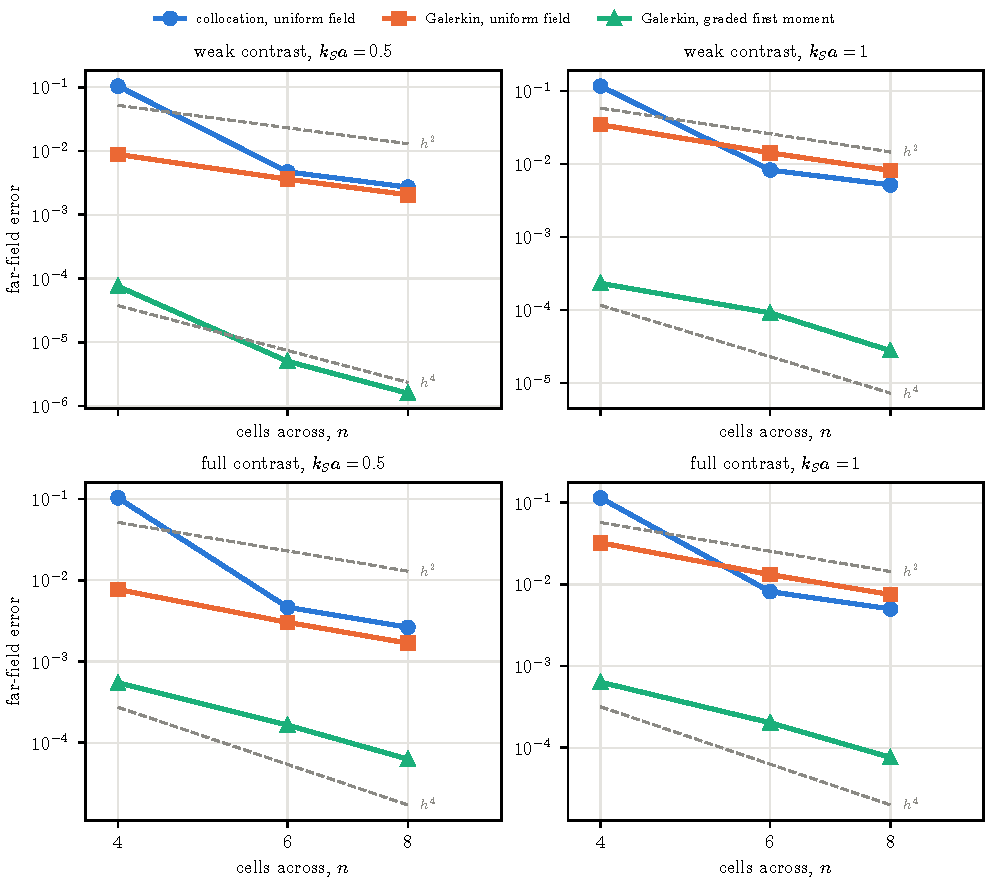
\includegraphics[width=\textwidth]{figures/fig_orders.pdf}
\caption{Far-field error against the number of cells across the sphere, for the collocation and Galerkin
uniform-field voxels and the graded first-moment voxel; dashed guides show $h^2$ and $h^4$. Top: weak
contrast (the discretisation alone). Bottom: full contrast, with the graded voxel solved by FFT to $n=16$
(Table~\ref{tab:fft}).}\label{fig:orders}
\end{figure}

\paragraph{A convention the Born limit cannot see.} The shear entries of the source are engineering
stress $2\sigma_{pq}$: the contrast operator maps the engineering strain $\gamma_{pq}$ to
$2\Delta\mu\,\gamma_{pq}$, and the kernel's shear columns carry a factor $\tfrac12$. The far field must
take the tensor stress $\sigma_{pq}$ from them, half the entry. Radiating the entry itself doubles the
shear stress, and a P wave along a cell axis has no shear stress at Born order, so the weak-contrast test
cannot see it. It appears at second order, through the density--shear cross terms, as an error in $T_2$
that does not fall with refinement ($4.65\%$ and $4.05\%$ at $n=4$ and $6$, against $4.22\%$ and $1.31\%$
when the far field agrees with the kernel for every source component).

\section{Discussion}\label{sec:discussion}

\paragraph{What three dimensions change.} Two things differ from the layer. The lateral first moments are
now excited, and they couple through the near field of neighbouring cells; and the discrete source,
projected cell by cell, jumps by $O(h^2)$ across every face between cells, where in the layer only the
faces normal to the stratification exist. The Born term does not see either: its error is the quadrature
error of the source, and it is of fourth order. The multiple-scattering term sees both, but neither costs
an order: its apparent order rises towards four, and the full solve follows it (\S\ref{sec:sphere}). The
approach is slow where few cells span the variation of the contrast, and does not depend on the frequency
or on the smoothness of the profile. The error of the multiple-scattering term is the defect
(\ref{eq:defect}) of the profile's projection onto the cells' field functions (\S\ref{sec:sphere}), a
static quantity three orders of magnitude above the Born term's error at these frequencies.

\paragraph{Galerkin and collocation.} With the lattice couplings then available, a uniform-field Galerkin
cell was measured several times worse than the collocation cell \citep{NestorContinuum2026}. Here, with every
block computed exactly, the uniform-field Galerkin voxel is comparable to the collocation voxel at second
order, and the graded Galerkin voxel is far better. The double average is the route to fourth order when
the coupling is exact.

\paragraph{Cost.} The linear cell has 36 unknowns against 9, the quadratic cell 90. On the sphere at full
contrast the linear cell reaches $7.6\times10^{-5}$ with $14{,}688$ unknowns at $k_Sa=1$; the collocation
voxel reaches only $4.2\times10^{-4}$ with $64{,}872$. The quadratic cell reaches $6.3\times10^{-6}$ with
$36{,}720$ unknowns where the linear cell needs $99{,}936$ for $4.9\times10^{-6}$. With an FFT
matrix-vector product the quadratic cell's kernel has $90\times315$ entries per offset against
$36\times90$, and at $n=12$ the solve takes $587$\,s and $6.8$\,GB on a workstation. The blocks of the
self cell and its neighbours are universal constants times powers of $h$ and $k$ (\S\ref{sec:moments})
and are computed once; the blocks between cells that do not touch cost a three-dimensional Gauss rule
over the eight pieces of the autocorrelation.

\paragraph{The representation of the medium.} The order of a cell is set by how well it represents the
medium, twice over: the contrast must be represented, and the field must be able to carry the variation
that the contrast imprints on it. A contrast of higher degree than the field is wasted; the measured gain
from it is $8\%$.

\section{Conclusions}\label{sec:summary}

A Galerkin cube that carries the mean and first moments of displacement and an independent strain, with a
contrast linear in the cell, converges at fourth order in its discretisation (at Born order) on a
three-dimensional body with an exact solution, where cells of constant properties converge at second. At
full contrast it is between one and two orders of magnitude more accurate than a uniform-field voxel at
the same cell size, and its error there has one identified source: the multiple-scattering term loses the
defect of the $L^2$ projection of the contrast onto the cell's field functions, a static quantity that
predicts the error to within $6\%$ and that explains the slow approach of the apparent order to four. A
cube whose field and contrast are both quadratic removes the defect at that order. Its measured gain over
the linear cube, $4.1$ to $20.8$ between $4$ and $12$ cells across, is the ratio of the two defects, and
it reaches a given accuracy with several times fewer cells. A quadratic contrast alone does not.
The singular integrals of the coupling blocks are available in closed form, as a power series in the
wavenumber with universal coefficients built from three elementary master integrals; they agree with the
quadrature construction of the same blocks to $10^{-10}$. The far field of such a scheme must take the source's
engineering shear stress as the coupling kernel does; the Born limit along a cell axis cannot reveal a
mismatch there.

\bibliographystyle{unsrtnat}
\bibliography{references}

\end{document}
